\chapter{System Control}

\section{Firm grasping algorithm \& Force control}

\begin{center}
\begin{figure}[H]
\centering
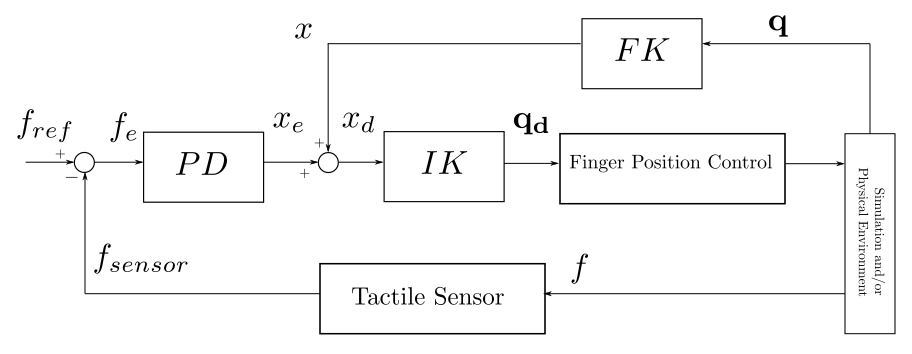
\includegraphics[width=12cm]{images/finger-force-control.png}\\
\caption{Force control on a Barrett Hand gripper finger}
\end{figure}
\end{center}

\section{Visual Servoing}

At this chapter we briefly investigate how visual servoing can be applied in surgery robotics. \textbf{Visual Servoing} is the use of visual information 
to guide and control a robot. The main task of visual servoing is to control the end-effector's pose using features extracted from visual information. The 
features that are usually extracted from cameras are the position and orientation of the detected object, the distance of the object from the camera (using 
stereoscopic vision, photogrammetry or other techniques), the size and the shape of the object. The visual servoing can be executed either in the robot's space 
using position-based servoing or in the camera's space (also known as "pixel space") by using the image-based technique.

\subsection{Position based servoing}

\begin{center}
\begin{figure}[H]
\centering
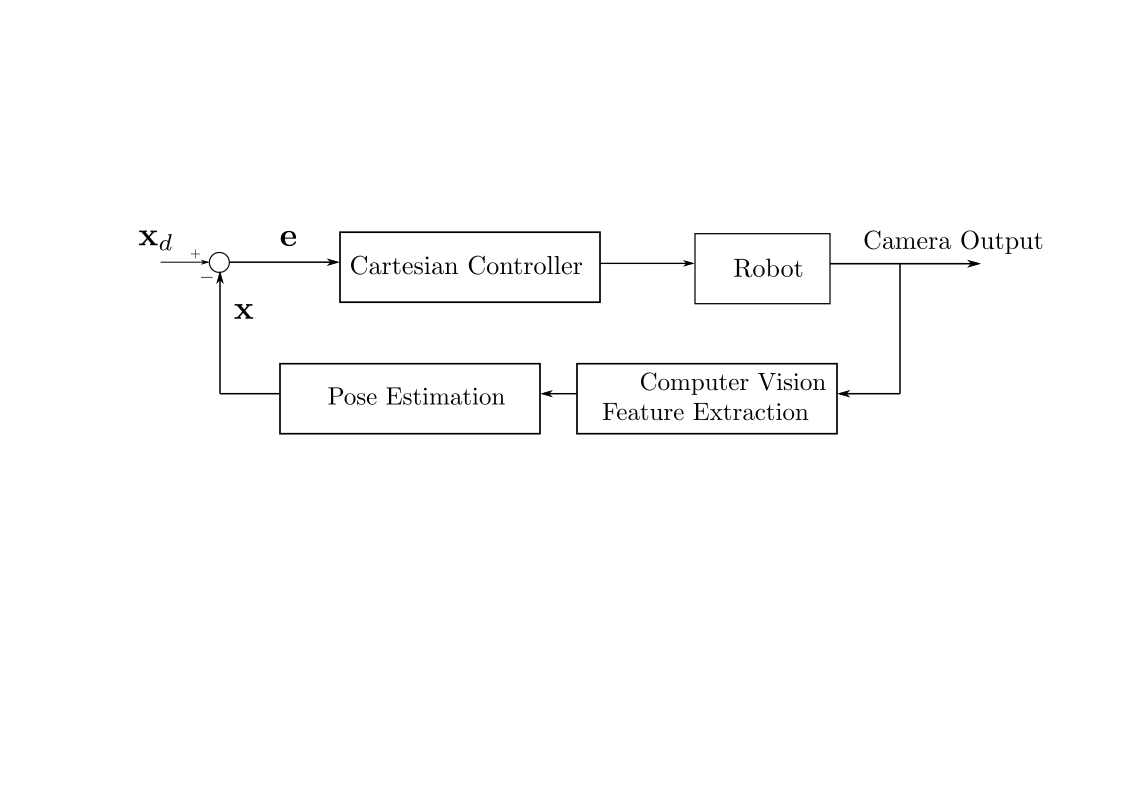
\includegraphics[width=0.8\textwidth]{images/visual-servoing-position-based.png}\\
\caption{Position based visual servoing closed loop control}
\end{figure}
\end{center}

\begin{itemize}
\item \textbf{Photogrammetric technique}
\item \textbf{Stereoscopic vision}: This methodology uses two separate views of the scene as taken from two viewports (from two cameras) 
and calculates the depth of various objects and areas using information from both views. For more details about stereoscopic vision see chapter \ref{stereoscopic-vision}
\item \textbf{Extracting depth from motion} This methodology is very similar to stereoscopic vision and is also known as \textit{monocular} or \textit{motion stereo}. The difference is that instead of using two views fromtwo distinct cameras this methodology 
uses two views from the same camera but from different points in time. A very important assumption for this methodology is to assume that two consecutive views from the video frame do not change significantly, so that some feature points can be matched in both views in order to calculate the depth information. This methodology 
is cheaper in terms of hardware but it fails to extract depth informations in cases where the robot is completely still.
\item \textbf{Servoing using 3D sensors}
\end{itemize}

\begin{center}
\begin{figure}[H]
\centering
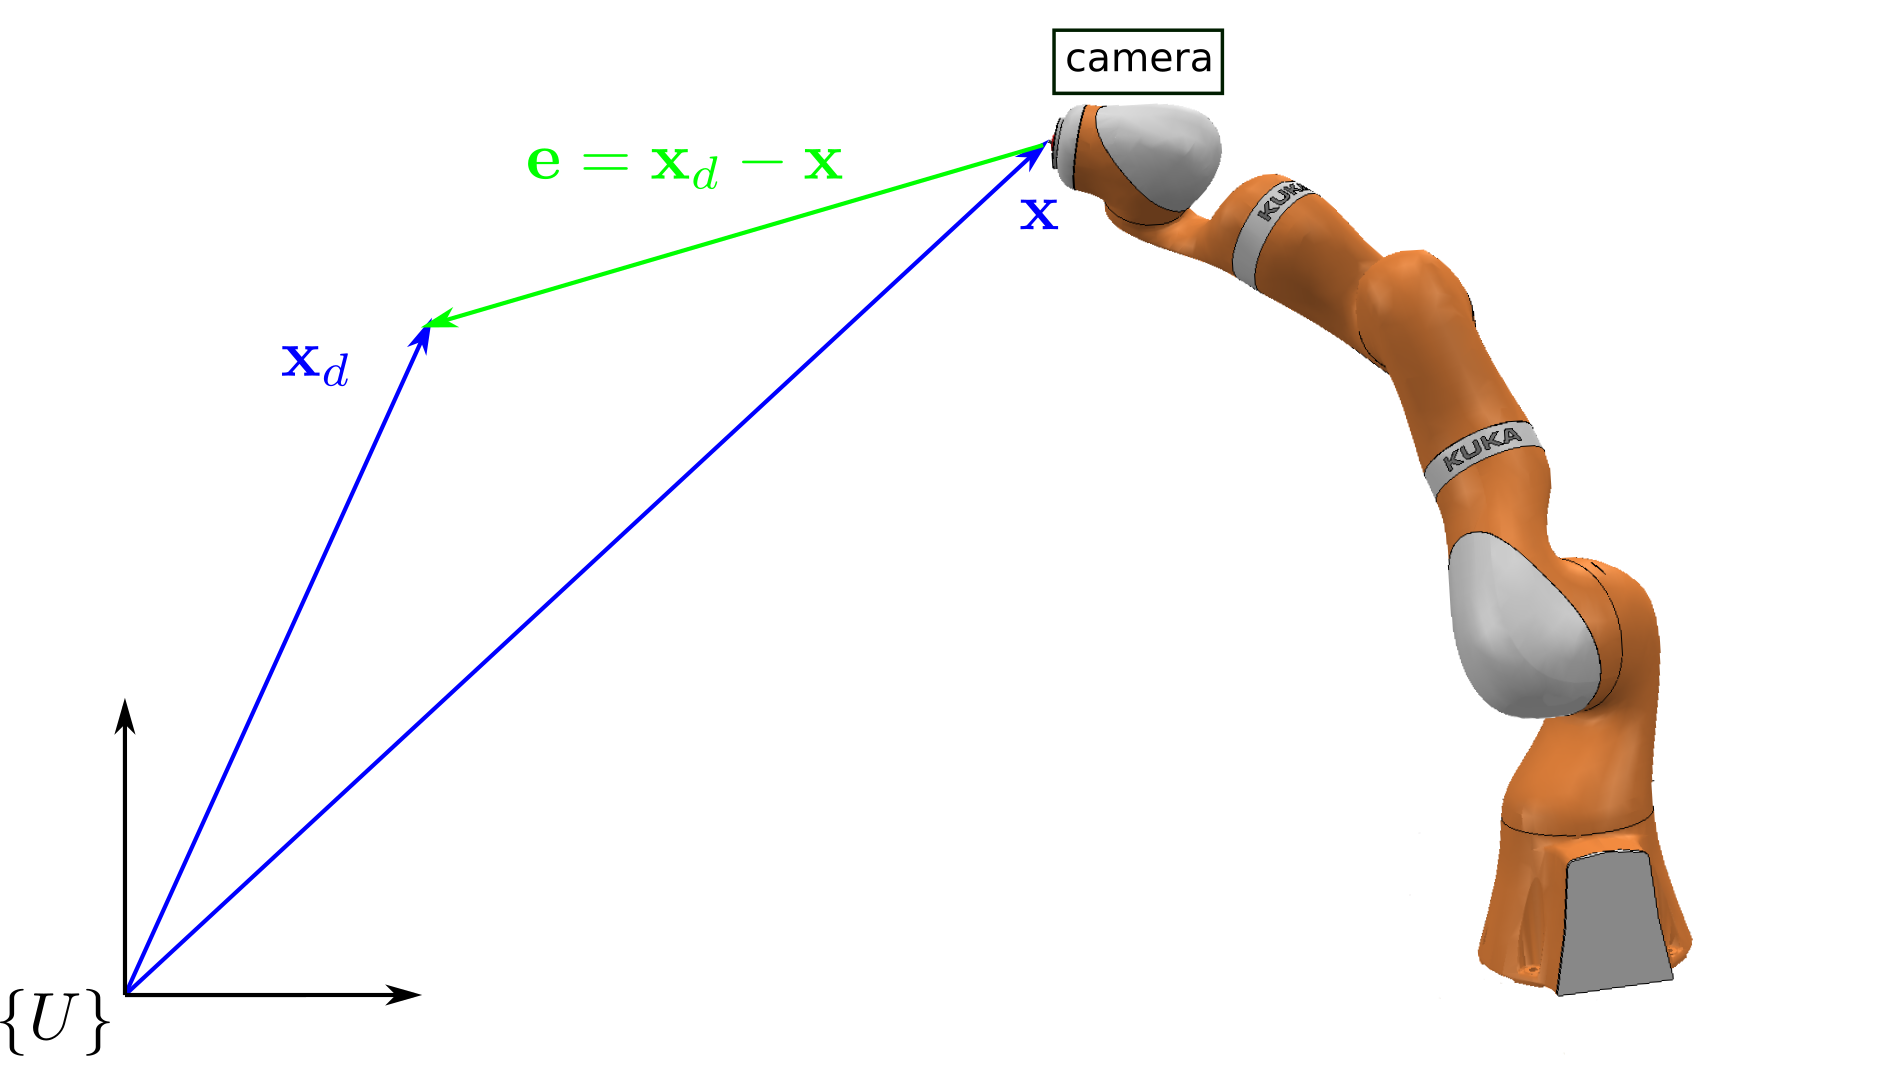
\includegraphics[width=0.6\textwidth]{images/visual-servoing-position-based2.png}\\
\caption{Position based visual servoing using depth from motion, stereo vision or 3D sensors, from which the desired position $\mathbf{x}_d$ is calculated and 
used to drive the robot.}
\end{figure}
\end{center}

\subsection{Image based servoing}

Image based servoing is a methodology for controlling a robot by directly using features extracted from the image as well as positions on the image plane. The goal of this methodology is 
to drive the robot in such a way so that the video frame is changed from an initial view to a final, desired view (see figure \ref{image-based-servoing-start-end} left and right frames). The commands 
that are sent to the robot from this methodology are defined in image space and not in the robot's task space. Moreover the distances calculated in image space are not directly related to distances 
in task space.

\begin{center}
\begin{figure}[H]
\centering
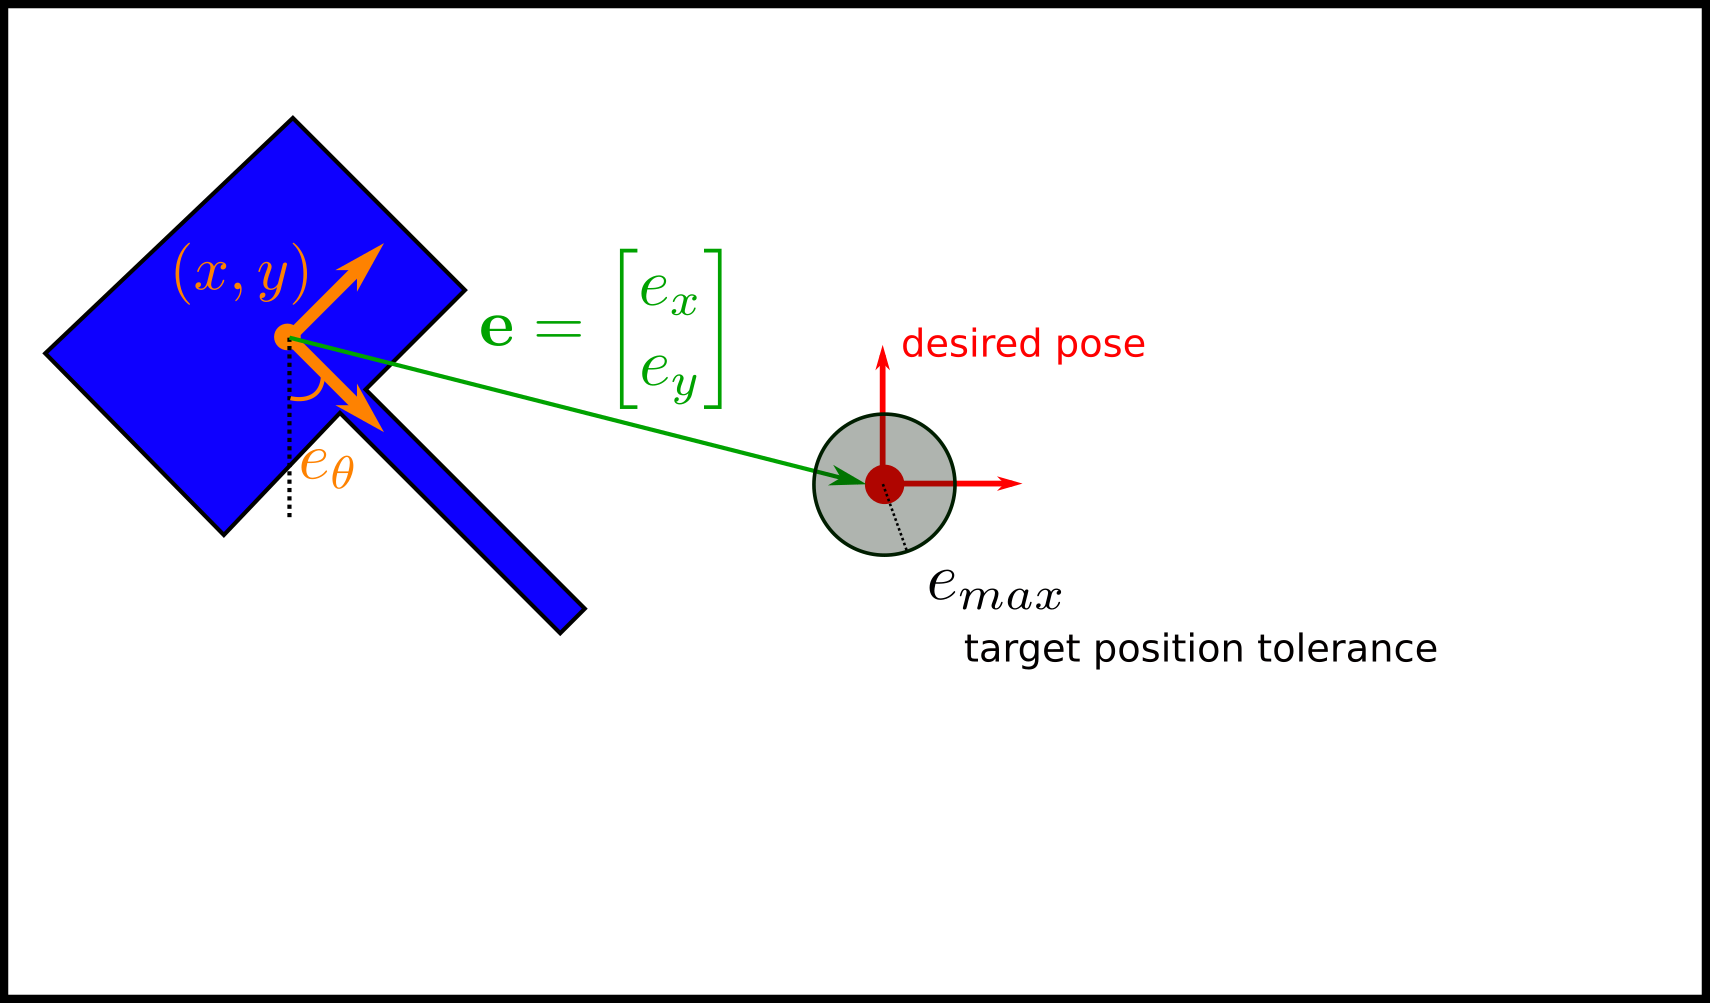
\includegraphics[width=0.45\textwidth]{images/visual_servo_start.png}
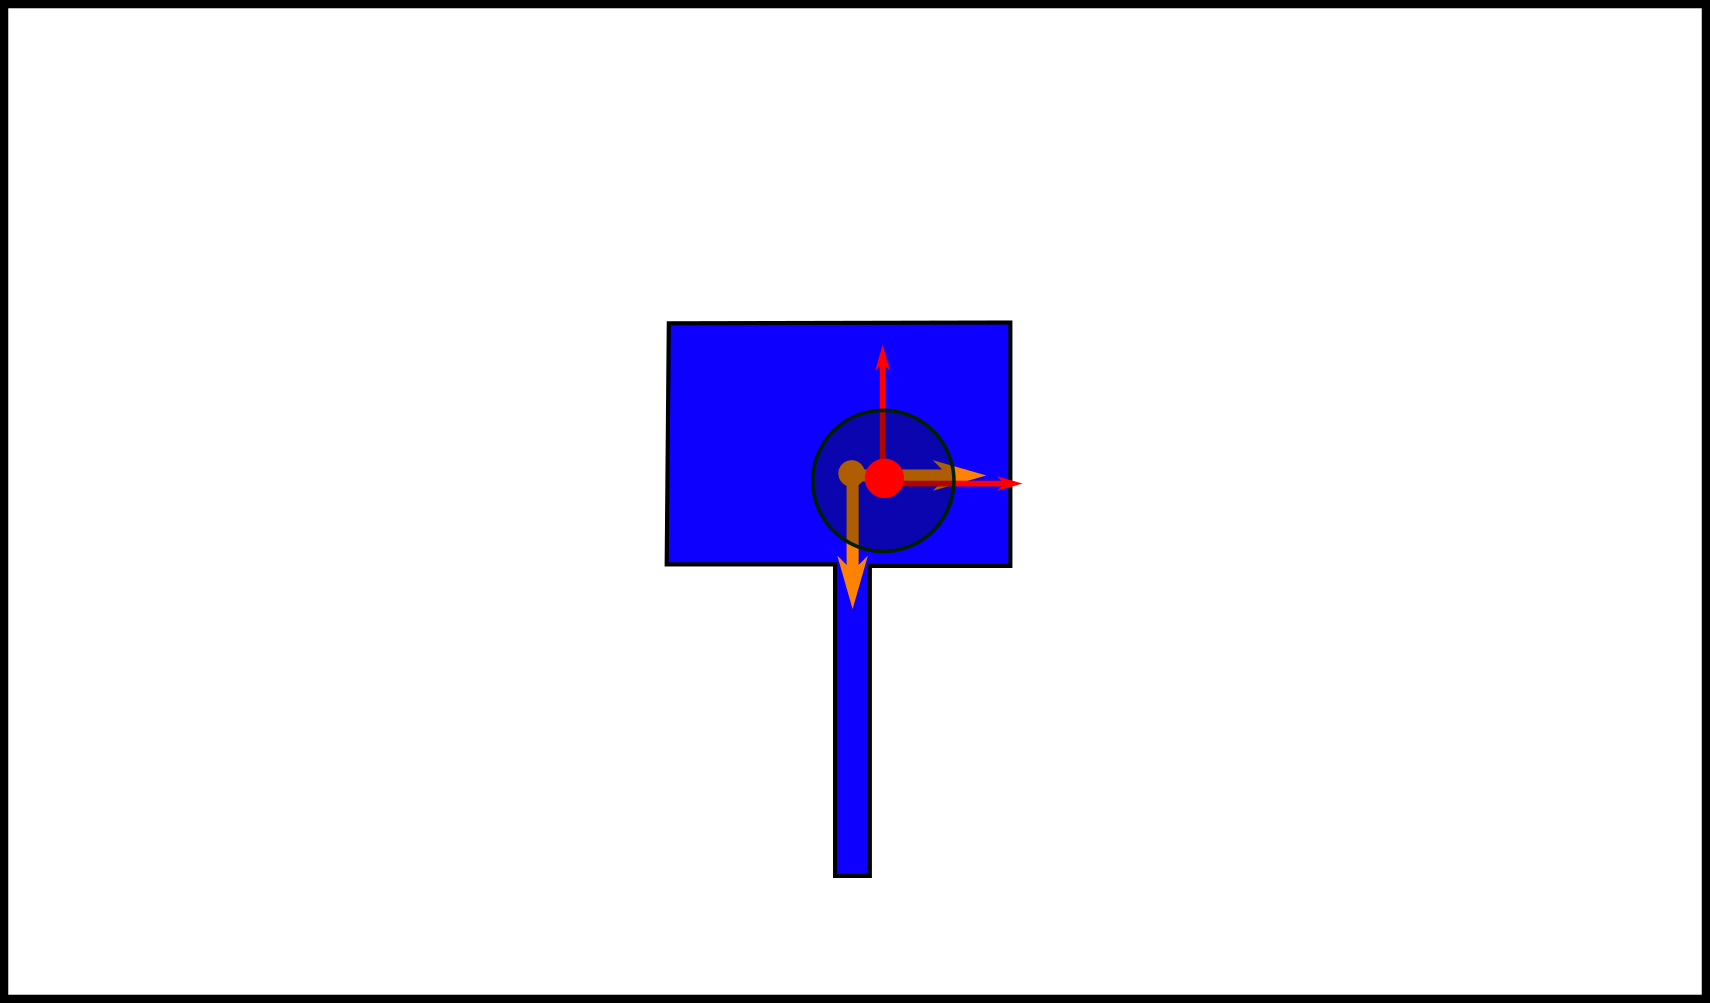
\includegraphics[width=0.45\textwidth]{images/visual_servo_end.png}\\
\caption{Image based visual servoing. The robot arm is controlled using the information gained from the video frames. The frames are 2Dimensional and thus 
the detected objects can have only 3 degrees of freedom which means we can mainly control 3 independent variables, here the $x,y,θ$ variables. The left image 
is the initial frame and the right image is the frame where the object is at the target pose.}
\label{image-based-servoing-start-end}
\end{figure}
\end{center}

The image based visual servoing control system as depicted in figure \ref{visual-servoing-image-based-control} consists of the \textbf{Image Controller}, the \textbf{Plant} (robot) and the \textbf{feedback term}. The Image controller is a simple 
\textbf{PD Controller} (PID can also be used, but in servo systems PD is more common) which outputs commands to be executed in the plant. These commands are not to be confused with the robot's internal controller commands. 
These commands are to be used to control the robot in task space, whereas the internal controller drives each joint to the desired angle. The feedback used to calculate the error for the controller, uses the camera's 
output and based on that it calculates the vector from the detected tool's center of mass to the center of the image frame (feature extraction).

\begin{equation}
\mathbf{x}[(k+1)T] = \mathbf{x}[kT] + \mathbf{u}[kT]
\end{equation}

where $\mathbf{x}[kT] = [x, y, z, θ, φ, ψ]^\top$ and the discrete PID control law is given by equation \ref{discrete-pid-control-law}
\begin{equation}
\label{discrete-pid-control-law}
\mathbf{u}[kT] = K_p \left[ \mathbf{e}[kT] + \frac{T}{T_i} \sum_{i=0}^{k-1} \mathbf{e}[iT] + \frac{T_d}{T} \left( \mathbf{e}[kT] - \mathbf{e}[(k-1)T] \right) \right]
\end{equation}

where $\mathbf{e}[kT] = [e_x, e_y, e_z, e_θ, e_φ, e_ψ]^\top$.

\begin{center}
\begin{figure}[H]
\centering
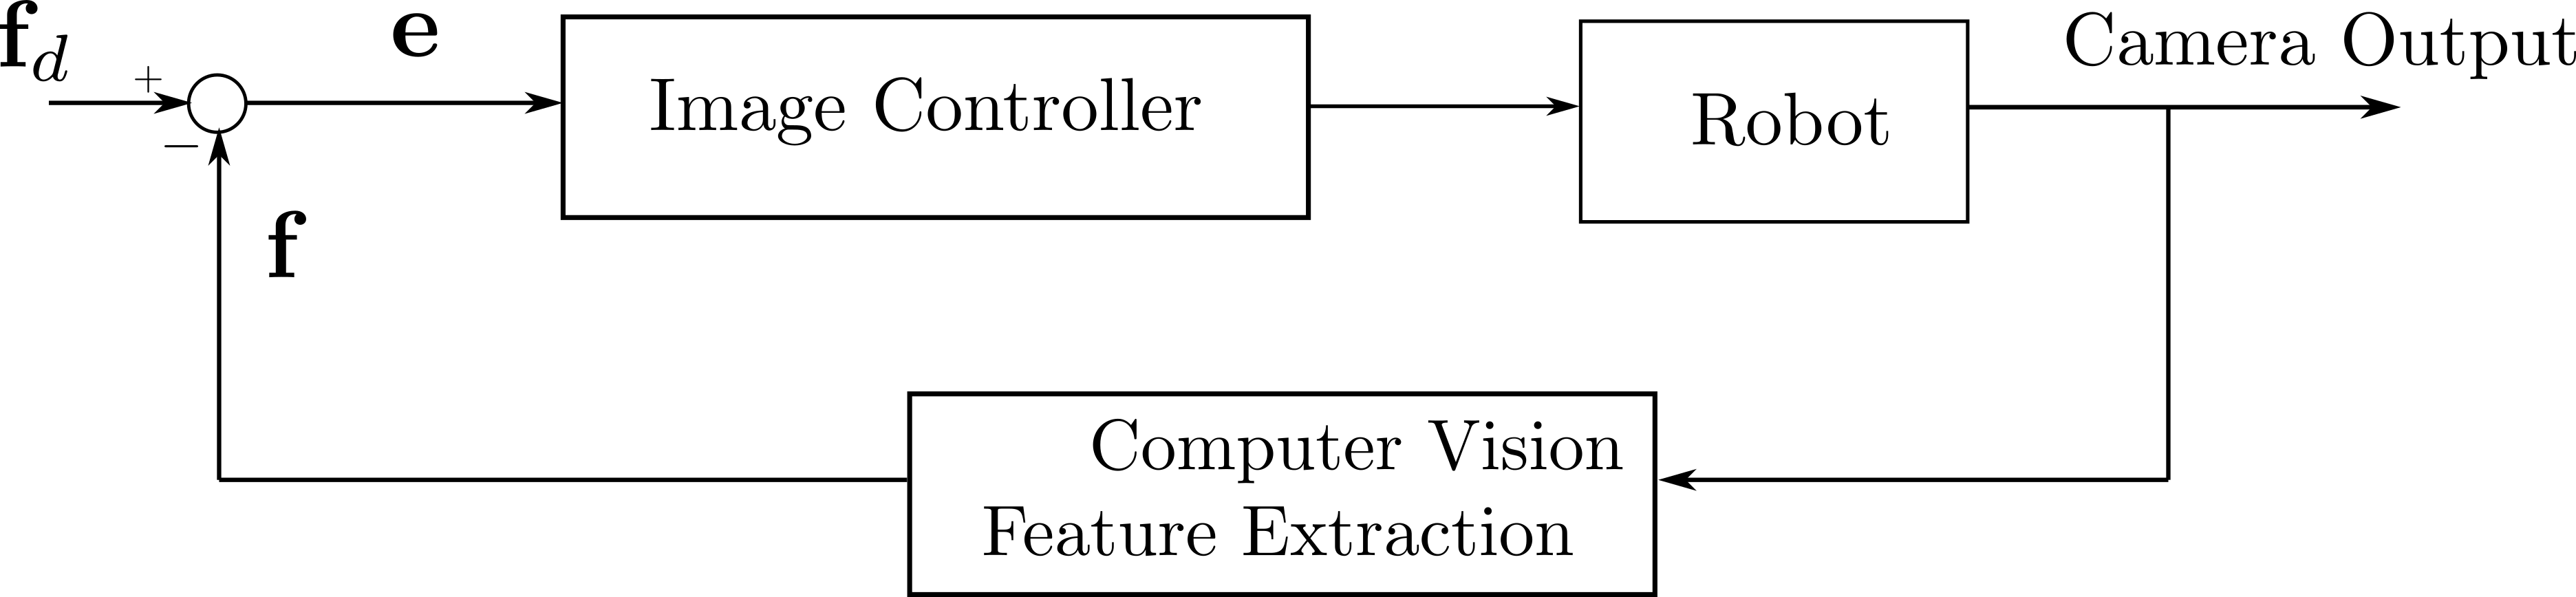
\includegraphics[width=0.8\textwidth]{images/visual-servoing-image-based.png}\\
\caption{Image based visual servoing closed loop control}
\label{visual-servoing-image-based-control}
\end{figure}
\end{center}
